%!TEX root = MemoireZelliges.tex

\makeatletter

% \newcommand{\partimage}[3][]{%
%   \gdef\@partimage{%
%     \settowidth{\imgwidth}{\includegraphics[#1]{#2}}
%     \vspace{6\baselineskip}
%     % \vfill
%     \small\itshape
%     \includegraphics[#1]{#2}\par
%     \parbox{\imgwidth}{\RaggedLeft#3}\par
%   }%
% }

\newcommand{\partimage}[3][]{%
  \gdef\@partimage{%
    \begin{tikzpicture}[
      remember picture, overlay, anchor=center,
      inner sep=0, outer sep=0.5mm,
      font=\small\itshape,
    ]
      \node (tab) at (current page.center) [shift={(0, -5)}] 
            {\includegraphics[#1]{#2}} ;
      \node [anchor=north east] at (tab.south east)
            {\RaggedLeft#3} ;
    \end{tikzpicture}
  }%
}

\renewcommand*{\beforepartskip}{\null\vskip 0pt plus 0.3fil}
\renewcommand*{\afterpartskip}{\vskip 0pt plus 0.7fil \newpage}
\renewcommand*{\printparttitle}[1]{%
  % \vfil\parttitlefont #1\vfil\vfil\@partimage\vfil%
  \parttitlefont #1\@partimage%
}



\renewcommand{\maketitle}{%
  % Entête
  \begin{tikzpicture}[
    remember picture, overlay, anchor=north,
    inner sep=0, outer sep=1cm,
  ]
    \node at (current page.north) {
      \begin{tikzpicture}
        \node (A) at (0.00, 0.00) [%
          draw, double distance=2pt, thick,
          text width=0.85\paperwidth, % align=right,
          inner sep=6pt,
        ] {%
          \begin{minipage}{5cm}
            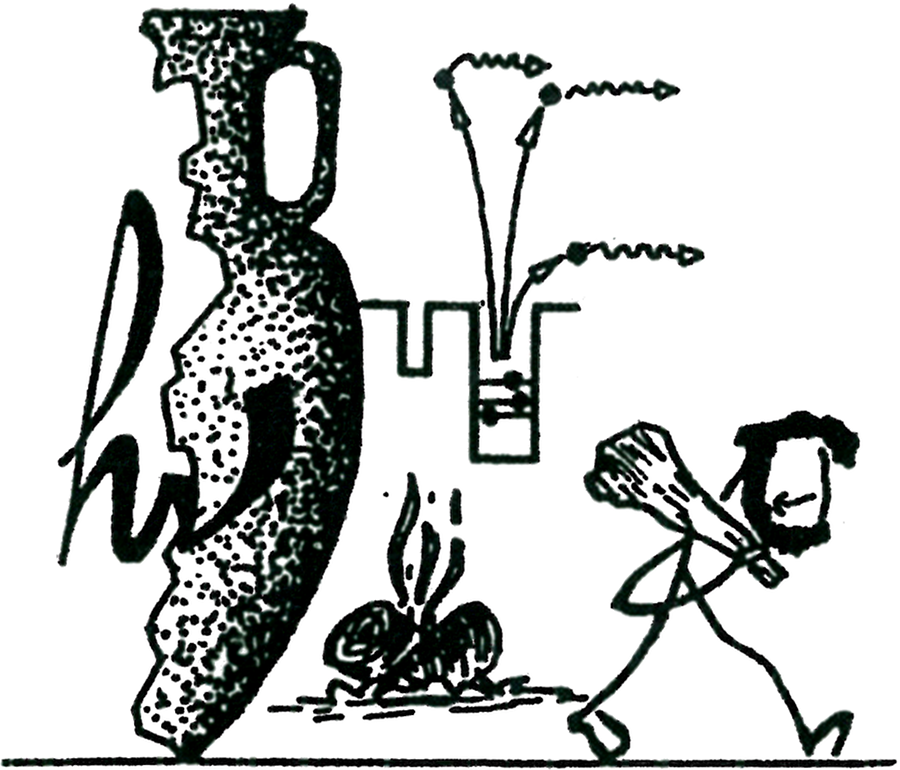
\includegraphics[width=5cm]{logo_CRPAA}
          \end{minipage}%
          \hfill%
          \begin{minipage}{12cm}
            \RaggedLeft
            Université de Bordeaux~3 -- Université de Bordeaux~1

            3\ieme~cycle -- \textbf{D.E.S.S.}\\
            \textbf{\larger\og MÉTHODES PHYSIQUES\\EN ARCHÉOLOGIE 
            ET MUSÉOGRAPHIE \fg}

            \medskip

            COMPTE RENDU DU STAGE DE RECHERCHE EFFECTUÉ AU\\
            \textbf{C.R.P.A.A.} \quad UMR CNRS~5060\\
            \textbf{C}entre de \textbf{R}echerche en \textbf{P}hysique 
            \textbf{A}ppliquée à L'\textbf{A}rchéologie\\
            \textbf{Maison de l'archéologie,} Esplanade des Antilles, 
            Domaine Universitaire,\\
            33607 - PESSAC cedex, FRANCE\\
            Tél. : 05.57.12.45.53 \quad Fax : 05.57.12.45.50
          \end{minipage}
        } ;
      \end{tikzpicture}
    } ;
  \end{tikzpicture}

  % Pied de page
  \begin{tikzpicture}[
    remember picture, overlay, anchor=south,
    inner sep=0, outer sep=1cm,
  ]
    \node at (current page.south) {
      \begin{tikzpicture}
        \node (F) at (0.00, 0.00) [%
          % below=1cm of E.south, 
          draw, thick, 
          text width=0.85\paperwidth, 
          inner sep=3pt,
        ] {%
          % \small Juin~2000 \hfill 
          \small \@date \hfill 
          MÉMOIRES DE LA SÉRIE \textbf{\frquote{FORMATION À ET PAR LA 
          RECHERCHE}} \hfill 
          \textbf{\no441.} DESS
        } ;
      \end{tikzpicture}
    } ;
  \end{tikzpicture}

  \begin{center}
    \vfill
    \vspace{5\baselineskip}

    {\LARGE
      Programme PACT ARCHI-MED Glaçures -- II\par
    }

    \rule{.5\textwidth}{1pt}

    {\bfseries\huge
      \MakeUppercase{Contribution à la réhabilitation architecturale 
      du \PaM, Meknès, Maroc, \siecle{17}}

      \bigskip

      % Recherche des caractéristiques physiques\\de zelliges de pavement
      \@title\par
    }

    \vfill

    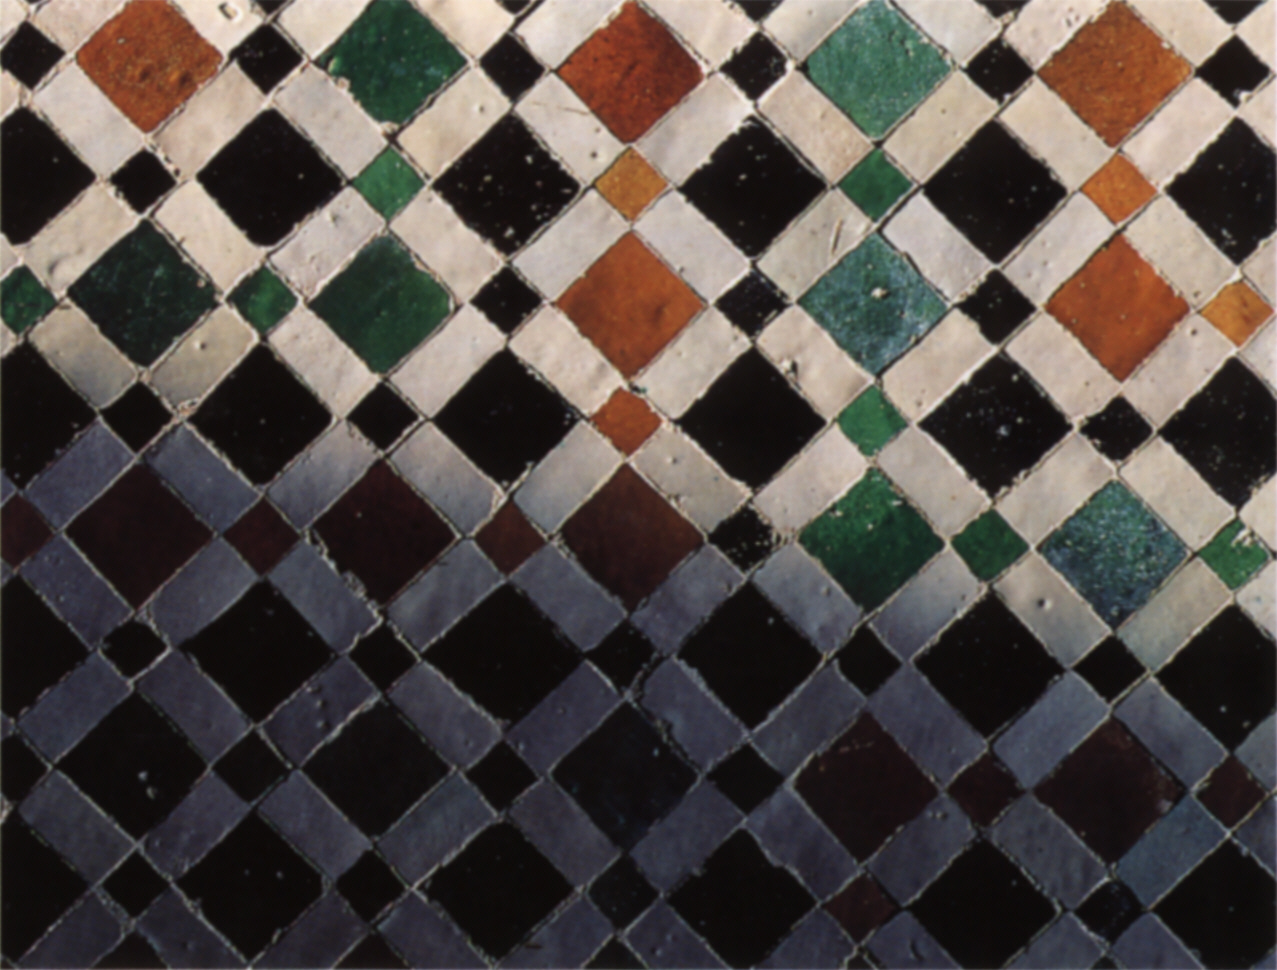
\includegraphics[width=11cm]{zellige_00}

    \vfill

    % \textbf{\Large\bsc{Labetoulle} Sonia}\par
    \textbf{\Large\@author}\par

    \emph{Maître ès Sciences\\(Chimie physique)}\par
  \end{center}
  \newpage
}
\makeatother
